The schematic for the Dual-Evaporator Subcritical Heat Pump cycle (SC2) is shown 
in Figure \ref{fig:SC2} and the corresponding operating conditions are summarized in Table 
\ref{tab:SC2_conditions}.

\begin{figure}[H]
    \centering
    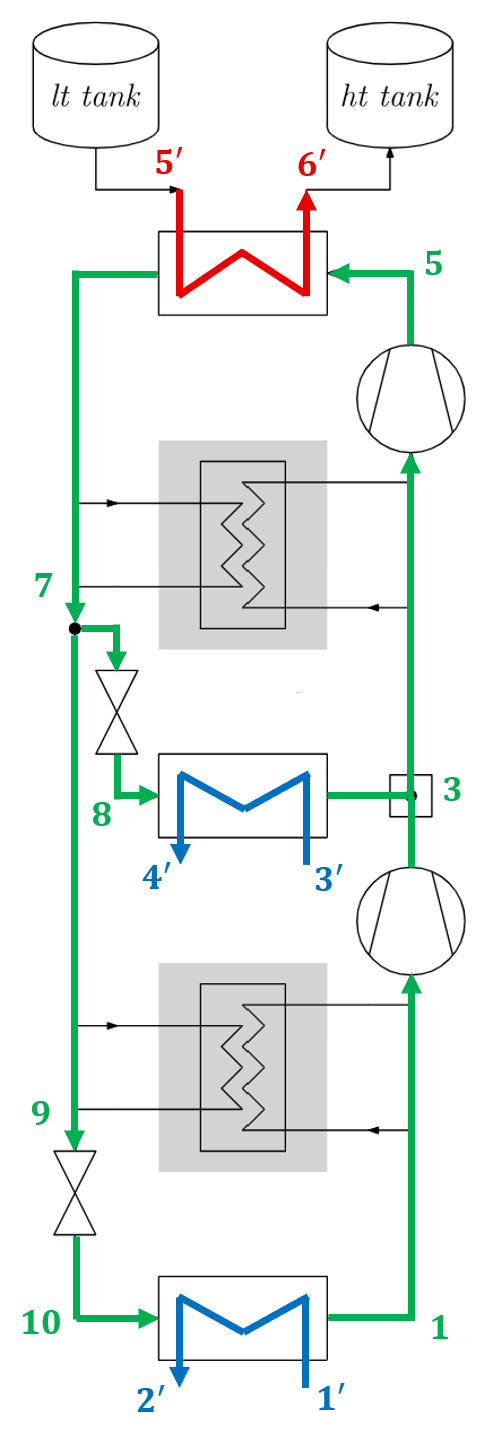
\includegraphics[width=0.35\textwidth]{Figures/SC2.png}
    \begin{minipage}{0.7\textwidth}
        \caption{Schematic of the Dual-Evaporator Subcritical Heat Pump cycle (SC2) 
        (\textit{green: working fluid; blue: heat source(s); red: heat sink})}
        \label{fig:SC2}
    \end{minipage}
\end{figure}

\begin{table}[H]
\centering
\begin{tabular}{|c|c|c|c|}
\hline
\textbf{LT heat source} & \textbf{MT heat source} & \textbf{Working fluid} & \textbf{Heat sink} \\
\hline
Water & Water & R290 (propane) & Water \\
%\hline
$T_{1}' = 10\,^{\circ}\mathrm{C}$ & $T_{3}' = 40\,^{\circ}\mathrm{C}$ & -- & $T_{5}' = 60\,^{\circ}\mathrm{C}$ \\
%\hline
$\dot{m}_\mathrm{c} = 0.4\,\mathrm{kg/s}$ & $\dot{m}_\mathrm{c} = 1.2\,\mathrm{kg/s}$ & -- & $\dot{m}_\mathrm{h} = 1\,\mathrm{kg/s}$ \\
\hline
\end{tabular}
\caption{Operating conditions for the SC2 cycle}
\label{tab:SC2_conditions}
\end{table}

\newpage